This chapter presents practical examples of PSHA done with the OQ-engine. By considering simple test cases,
the effect of the various modeling parameters is shown so as to better explain the underlying algorithms. Few
cases considering real PSHA models illustrates the capabilities of the OQ-engine when dealing with complex
models.

\section{Classical PSHA with an Area Source}
We consider here the case of a single area source. The source has a circular shape of 200 km radius. The activity
is described by a truncated Gutenberg-Richter magnitude frequency distribution, with minimum magnitude
equal to 5 and maximum magnitude equal to 6.5. The \textit{a-value} is 5 (i.e. the source generates one
event per year with $M \ge 5$) and \textit{b-value} is 1. The seismogenic layer extends from 0 to 20 km.
Ruptures are associated to a single hypocentral depth (10 km) and nodal plane (strike 0, dip 90, rake 0).

\subsection{The area source discretization step}
We study here the effect of the area source discretization step ($\Delta$) in the calculation of hazard map values. That is, we investigate the effect that the spacing used to discretize the region delimited by the area
source boundary has on hazard levels corresponding to a given probability of exceedance. We thus compute
hazard curves (for PGA) on a set of locations equally spaced by 10 km defing a profile crossing the centre of the area source, from east to west.
We compute hazard curves using different GMPEs (Boore and Atkinson 2008, Chiou and Youngs
2008, Campbell and Bozorgnia 2008 and Abrahamson and Silva 2008) to investigate the potential dependence of the results accuracy on the ground motion model. From the hazard curves we extract PGA values corresponding to 10 \% in 50 years. Results for four discretization levels (20, 10, 5, and 2.5 km) are show in
Figure \ref{fig:delta_area}. When using $\Delta=20$ km, the hazard map values show strong fluctuations
 (where the highest are for the Boore and Atkinson 2008 model) within the area region (that is in the distance
range [-200, 200] km). For discretization steps equal to or smaller than 10 km, the different solutions converge instead to the same values.
\begin{figure}
\centering
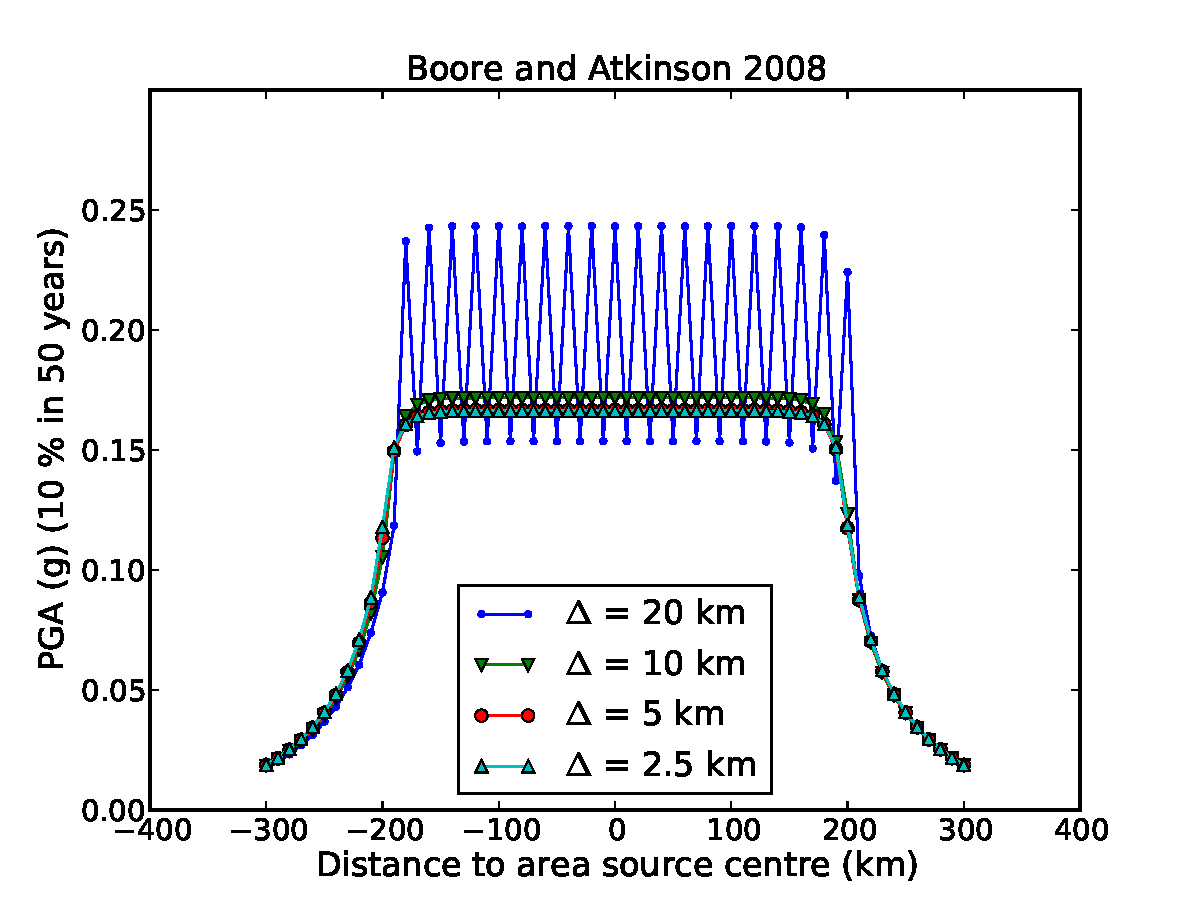
\includegraphics[width=7cm]{./Pictures/PGA_0pt1_source_model_a5_BA2008.pdf}
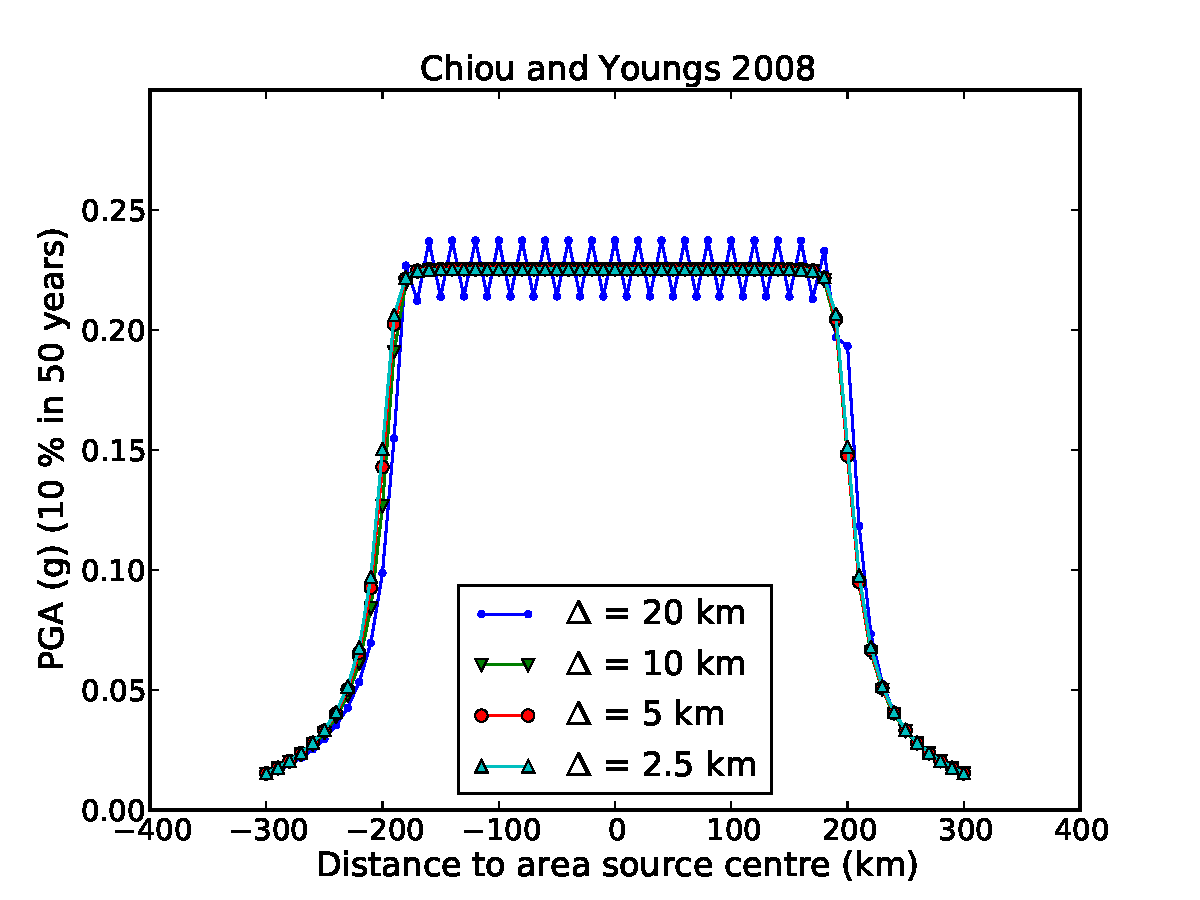
\includegraphics[width=7cm]{./Pictures/PGA_0pt1_source_model_a5_CY2008.pdf}
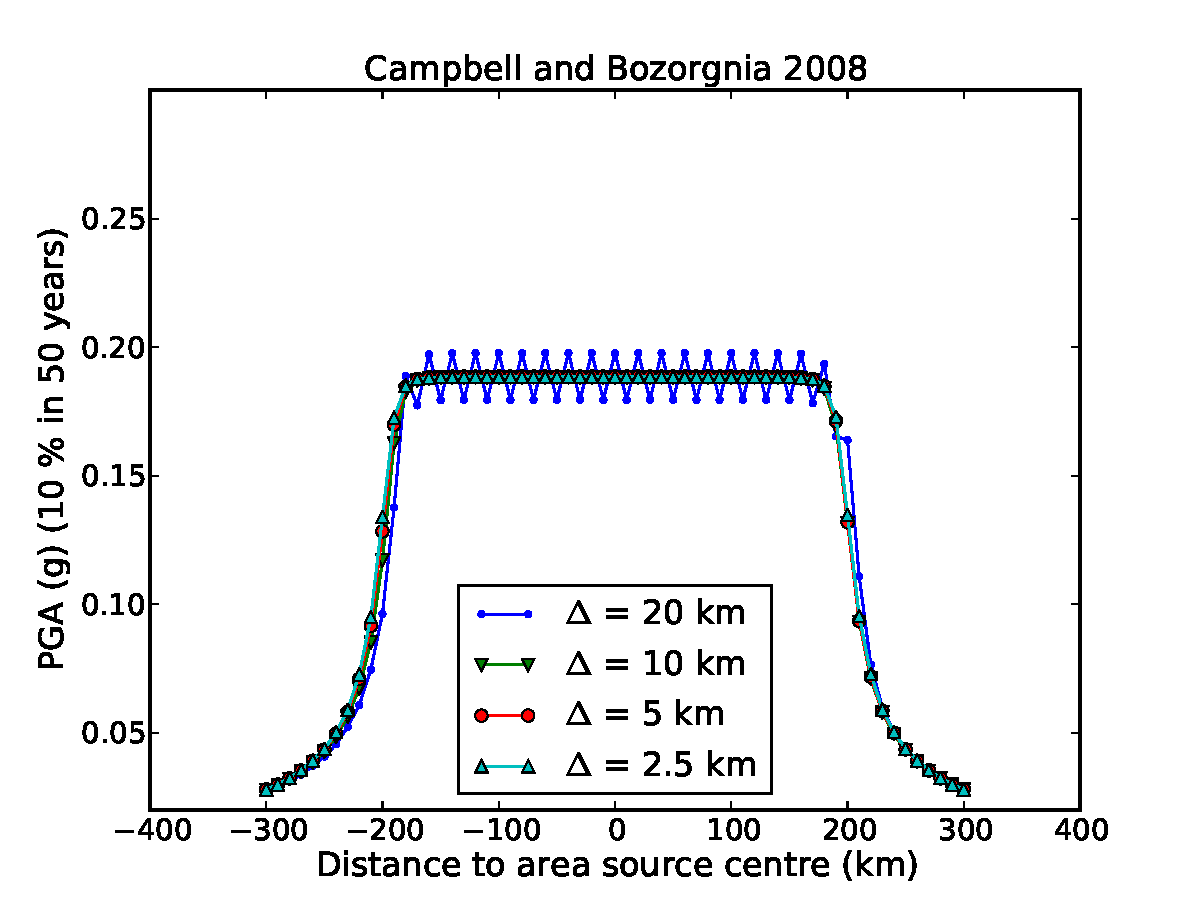
\includegraphics[width=7cm]{./Pictures/PGA_0pt1_source_model_a5_CB2008.pdf}
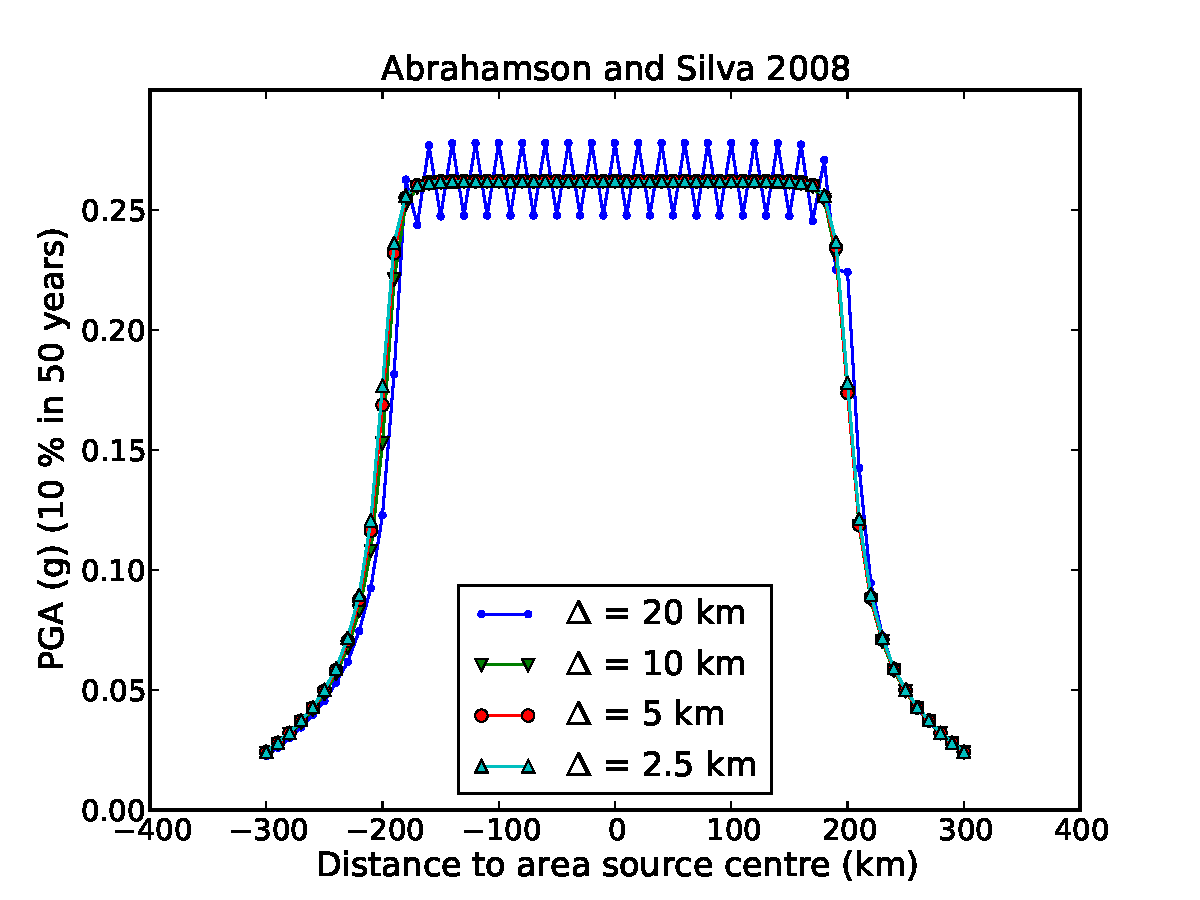
\includegraphics[width=7cm]{./Pictures/PGA_0pt1_source_model_a5_AS2008.pdf}
\caption{The effect of the area source discretization step ($\Delta$) on hazard map calculation}
\label{fig:delta_area}
\end{figure}

\subsection{The effect of dip and rake angles}
To investigate the effect of modelling earthquake ruptures with different inclination (that is dip angle) and
faulting style (rake angle), we compare here hazard map values for an area source generating only vertical,
strike-slip ruptures and an area source generating dipping (dip=$50^{\circ}$), reverse (rake=$90^{\circ}$) ruptures.
To investgate the potential dependence on the source seismic activity level, we compute hazard maps for
area sources having different Gutenberg-Richter a values ($a_{GR}$) equal to 3, 4 and 5, corresponding to
annual occurrence rates above $M=5$ of 0.01, 0.1 and 1, respectively. Results are shown in Figure \ref{fig:dip_rake_area}. Sensitivity on rupture dip and faulting style clearly depends on the source activity level and on the GMPE model. Indipendently of the GMPE, the highest absolute difference in PGA is for $a_{GR}=5$. Among the different GMPE models, Campbell and Bozorgnia 2008 shows the highest sensitivity (about 20 %
increase in PGA at $a_{GR}=5$), while Boore and Atkinson 2008 shows the lowest sensitivity.
\begin{figure}
\centering
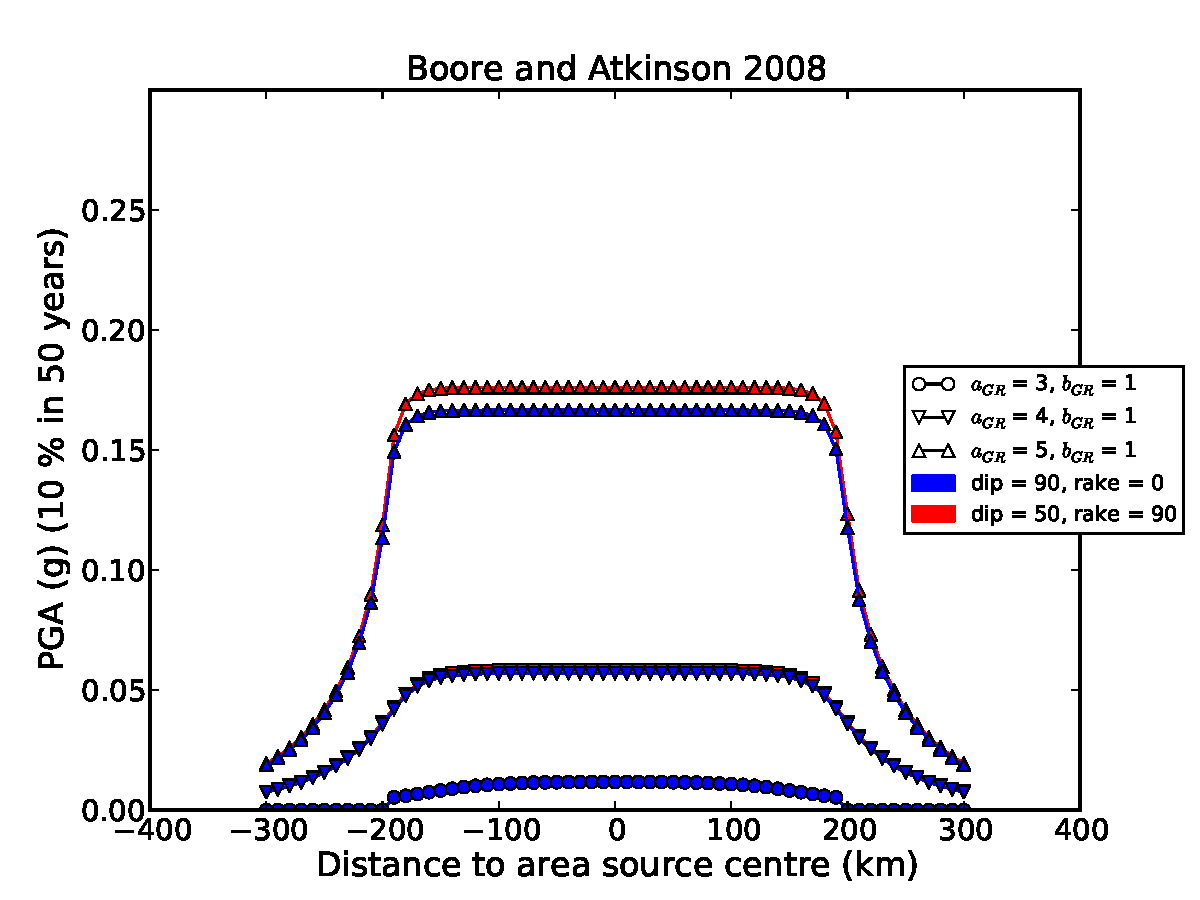
\includegraphics[width=7cm]{./Pictures/PGA_0pt1_BA2008_dip_rake.pdf}
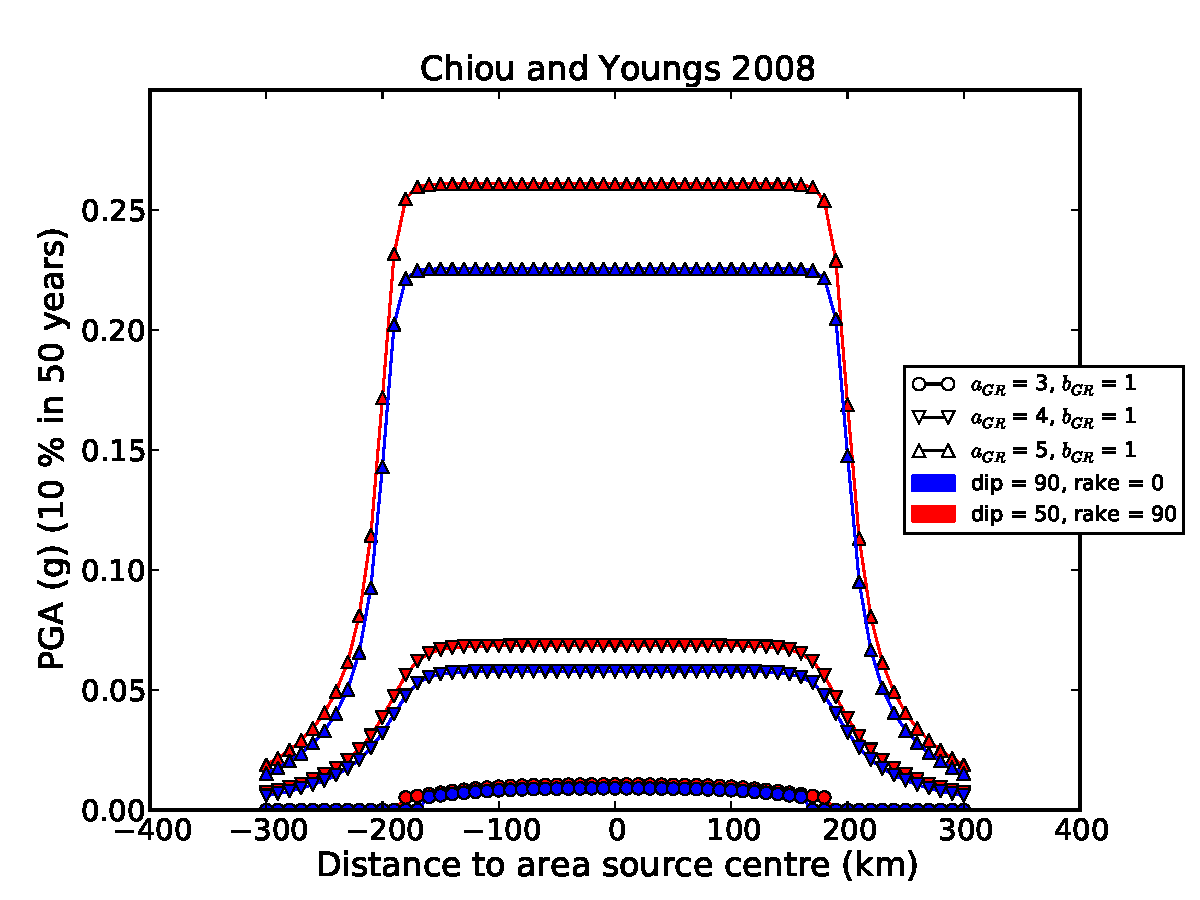
\includegraphics[width=7cm]{./Pictures/PGA_0pt1_CY2008_dip_rake.pdf}
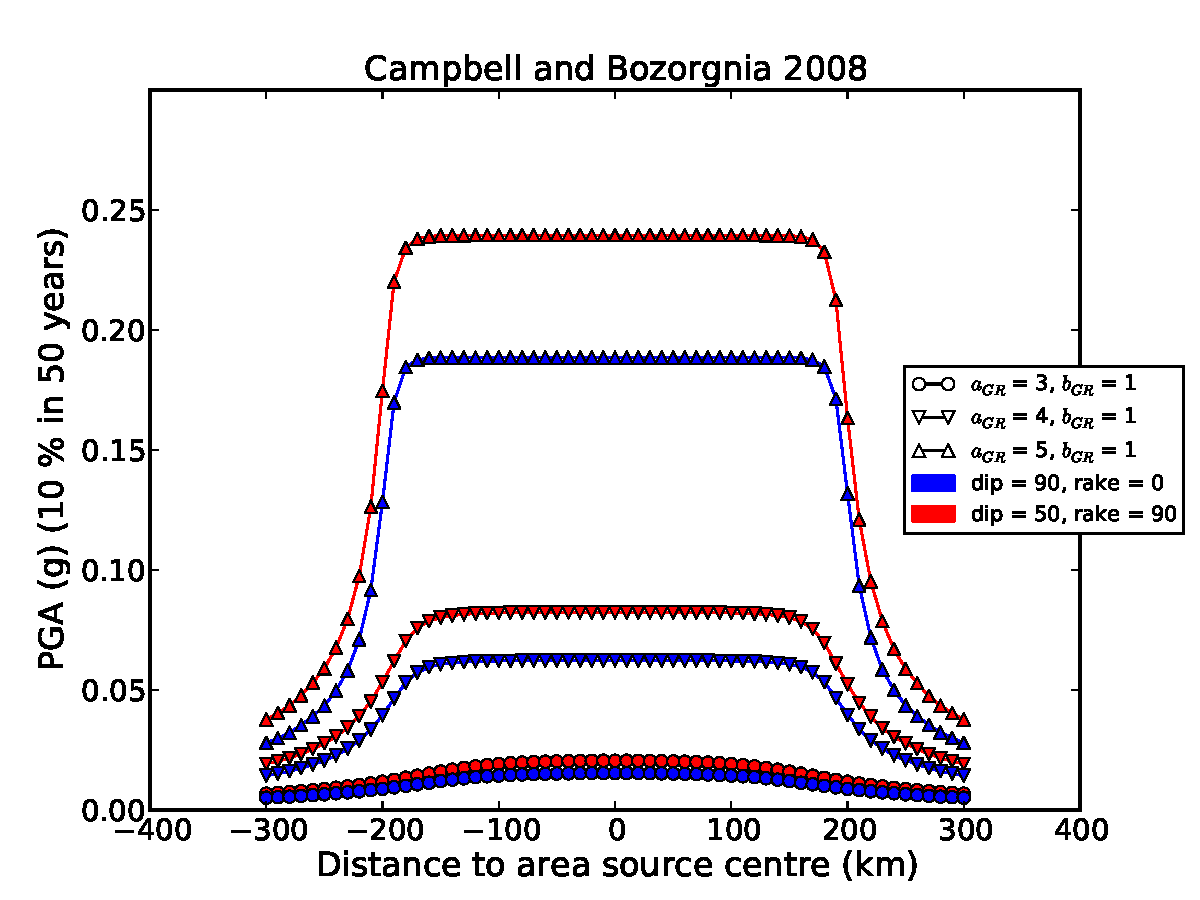
\includegraphics[width=7cm]{./Pictures/PGA_0pt1_CB2008_dip_rake.pdf}
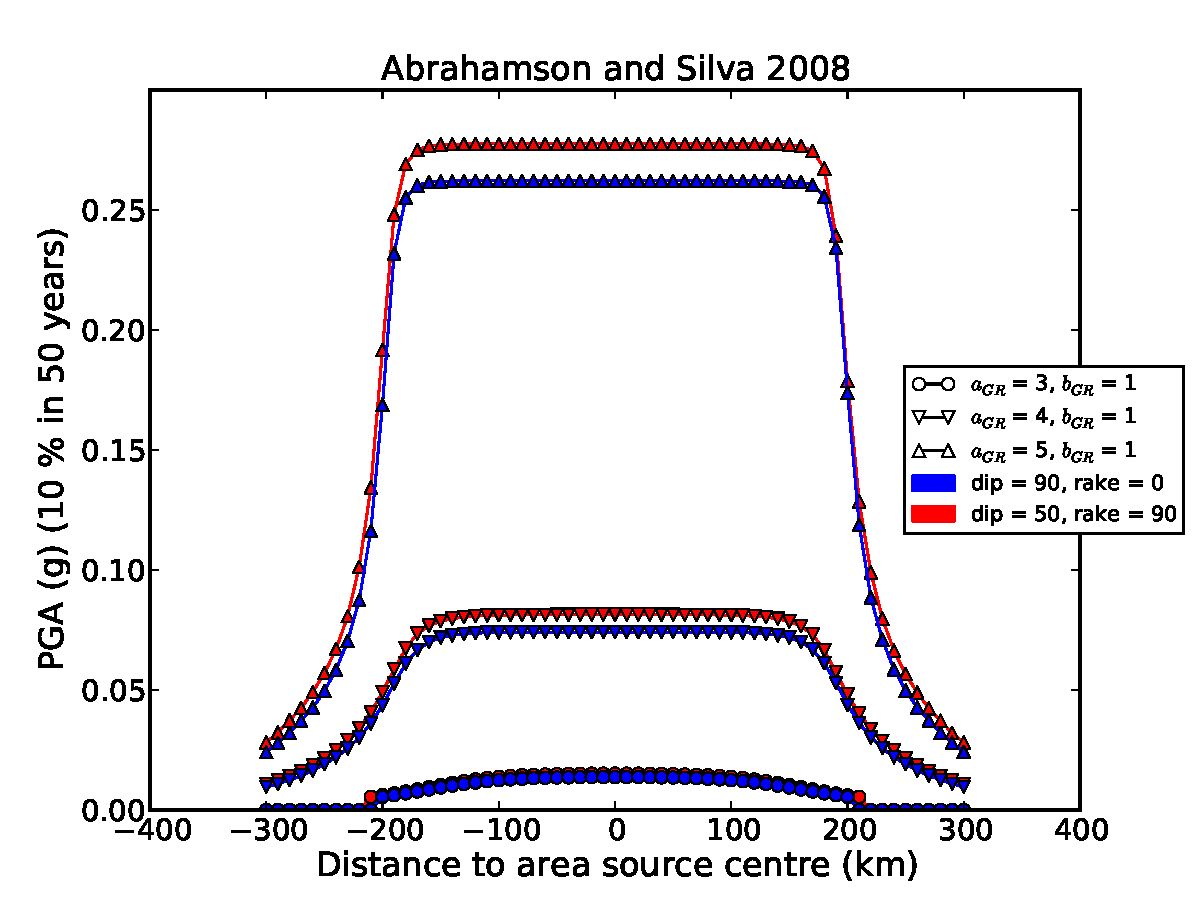
\includegraphics[width=7cm]{./Pictures/PGA_0pt1_AS2008_dip_rake.pdf}
\caption{The effect of dip and rake angles on hazard map calculation.}
\label{fig:dip_rake_area}
\end{figure}

\subsection{The effect of the hypocentral distribution}
Another modeling parameter which can influence hazard estimates from an area source is the hypocentral
depth distribution. We show here the effect of considering a single hypocentral depth value (10 km) versus
considering a set of normally distributed values with mean $\mu=10$ km and standard deviation $\sigma=4$ km. By considering the same source-sites configuration as in the previous analysis, and vertical
strike-slip ruptures with single strike ($0^{\circ}$), we compute hazard maps considering two $a_{GR}$ values (4 and 5). We use the GMPE model of Campbell and Bozorgnia 2008. Figure \ref{fig:hypo_depth_area} shows hazard map values along the site profile for different
return periods (RP) and $a_{GR}$ values. The effect of the distribution of hypocentral values becomes visible when considering long return periods (50000 years) and increases with increasing $a_{GR}$.
\begin{figure}
\centering
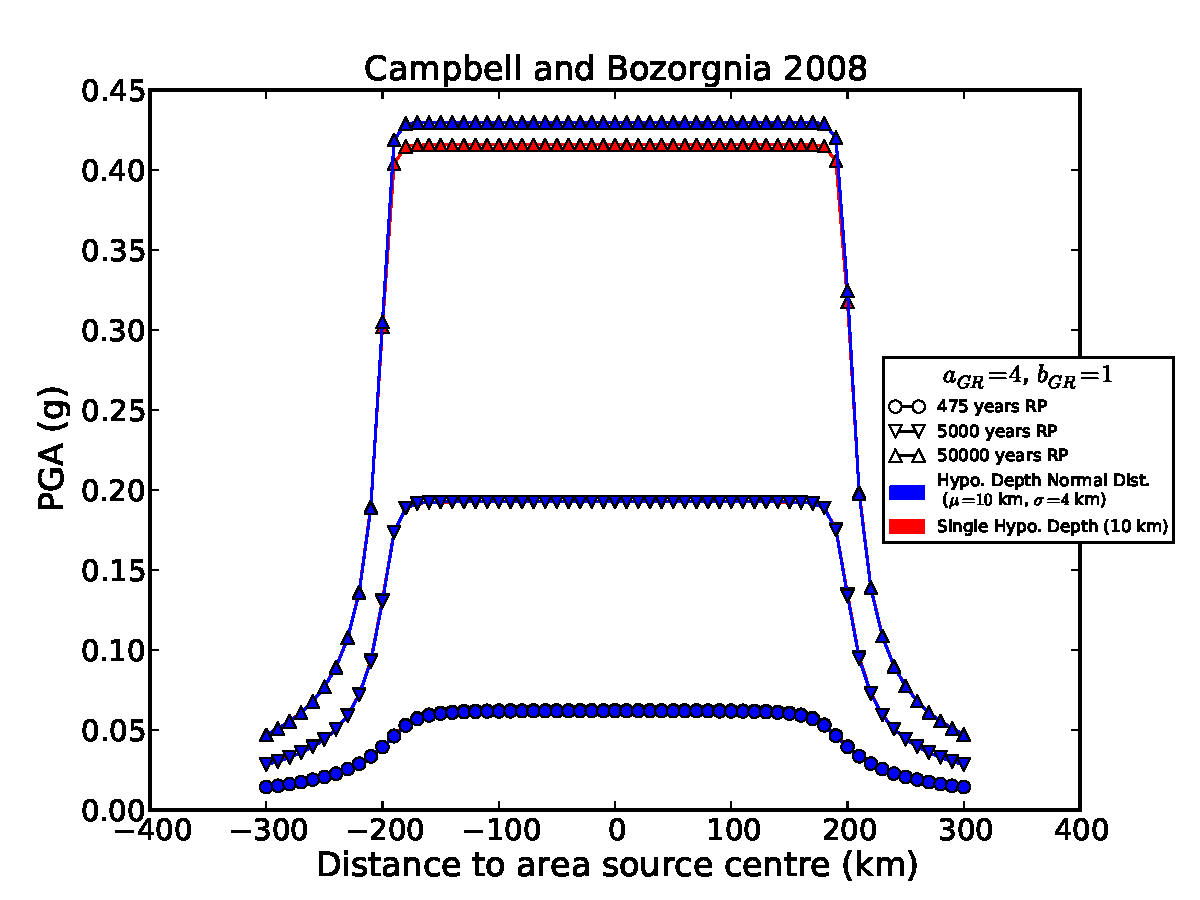
\includegraphics[width=7cm]{./Pictures/PGA_a4_CB2008_hypo_depth.pdf}
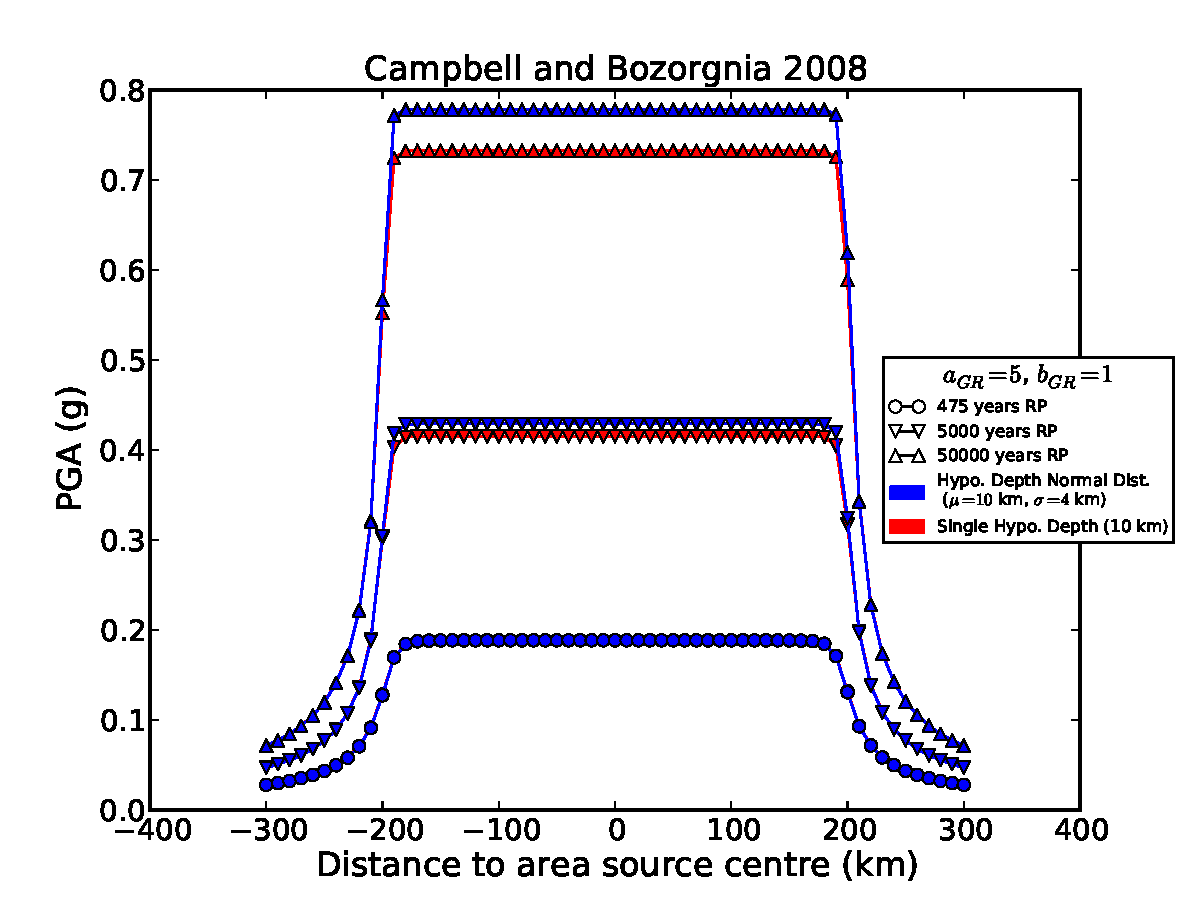
\includegraphics[width=7cm]{./Pictures/PGA_a5_CB2008_hypo_depth.pdf}
\caption{The effect of hypocentral depth on hazard map calculation.}
\label{fig:hypo_depth_area}
\end{figure}


\section{Classical PSHA with complex logic tree}
We consider here a synthetic case of a classical PSHA calculation based on a simple source model consisting of 5 identical area sources. Each source has a square shape of $0.5^{\circ}$ side. Four sources are arranged to form a regular mesh. The fifth source is placed in the middle of the mesh and overlaps with the other
four sources. Each source, however, can have 5 possible ($a_{GR}$, $b_{GR}$) pairs and 3 possible
maximum magnitudes. Assuming the uncertainties to be uncorrelated among sources, the total number of
possible source parameters combinations can be written as:
\begin{align}
N = N_{GR}^{N_{S}} \times N_{MaxMag}^{N_{S}}
\end{align}
where $N_{GR}$ is the number of Gutenberg-Richter parameters (i.e. $a_{GR}$ - $b_{GR}$ pairs) for each
source, $N_{MaxMag}$ is the number of maximum magnitudes for each source, and $N_{S}$ is the number
of sources. In the present case $N_{GR}=5$, $N_{MaxMag}=3$, $N_{S}=5$, and thus $N=5^{5} \times 3^{5}=759375$. $N$ represents the total number of paths in the source model logic tree.\\
The OQ-engine allows random sampling the logic tree to avoid calculating hazard results for all possible
logic tree paths. Figure \ref{fig:logic_tree_curves} presents mean and quantile hazard curves
as obtained from different numbers of samples (10, 100, 1000, 5000). It can be seen how, by increasing the number
of samples, results tend to converge to similar values. Indeed, curves obtained from 1000 and 5000 samples are almost indistinguishable. The Monte Carlo sampling offers therefore an effective way to reduce the computational burden associated with a large logic tree and to still obtain reliable results. The stability of the
results can be always controlled by perfoming a convergence analysis to identify the number of samples
which are required to obtain values that are stable within a certain tolerance level.
\begin{figure}
\centering
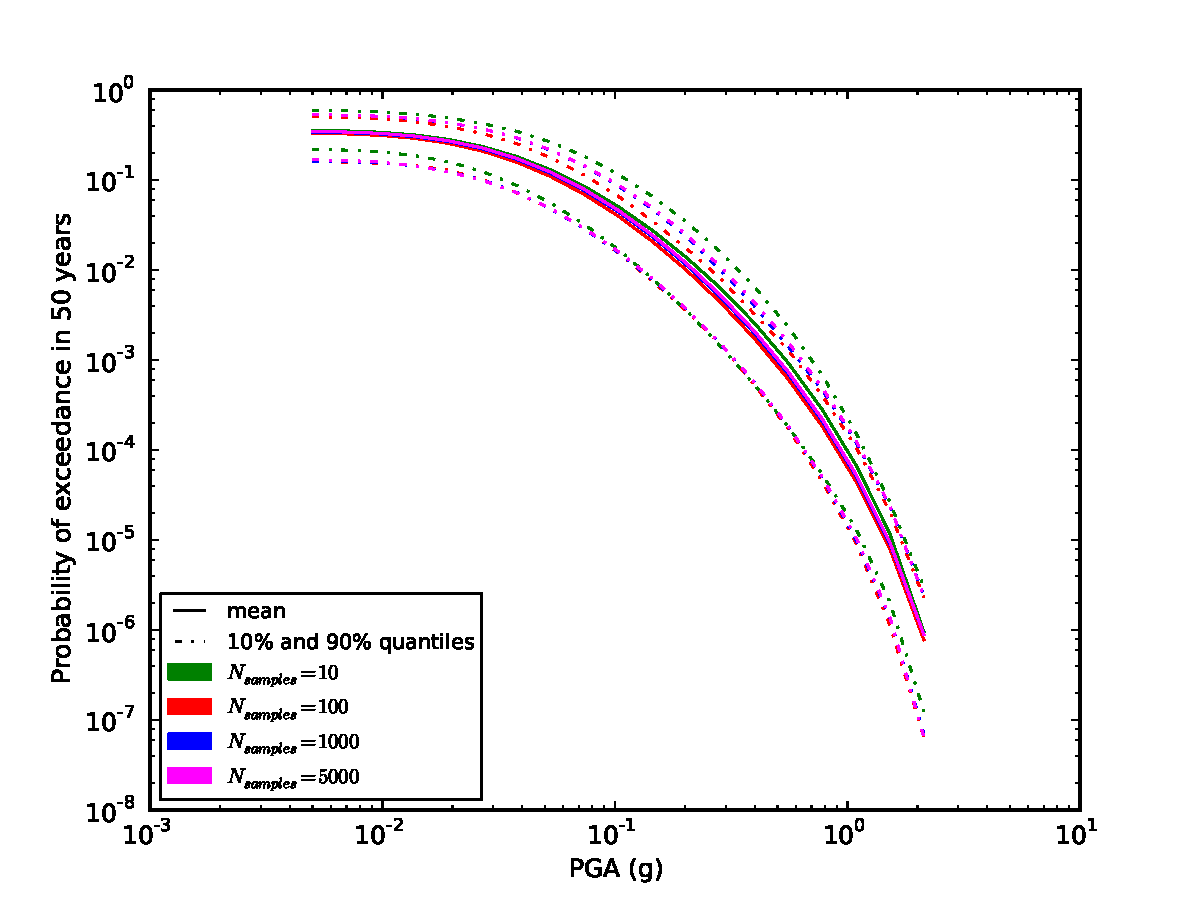
\includegraphics[width=14cm]{./Pictures/LogicTreeCurves.pdf}
\caption{Mean and quantile hazard curves obtained from Monte Carlo sampling of logic tree.}
\label{fig:logic_tree_curves}
\end{figure}

\section{Convergence between Classical and Event-based PSHA}
The event based approach allows generating stochastic event sets and ground motion fields which can then
be used to reproduce the classical results. We present here an event-based calculation for a location corresponding to the city of Seattle. The calculation is done using the 2008 seismic hazard model for conterminuos U.S. (CITE PETERSEN et al. 2008). A stochastic event set corresponding to a duration of 10000
years is generated (Figure \ref{fig:seattle_ses}). The event set contains earthquake ruptures within a radius of
200 km from the city of Seattle (longitude = 122.3W, latitude = 47.6N). The event set includes large subduction interface earthquakes generated in the Cascadia region, as well as deep intraslab and shallow active crust earthquakes. From each event, ground shaking values are simulated in the city of Seattle (considering the full set of GMPEs prescribed by the model). From ground motion values, the mean
hazard curve (probability of exceedance in 50 years) for PGA is computed, and compared against the
one obtained using the classical approach (Figure \ref{fig:seattle_curves}). The curve obtained can reliably
reproduce the probabilities of exceedance down to $10^{-2}$. For lower probabilities a stochastic event
set with longer duration is required.
\begin{figure}
\centering
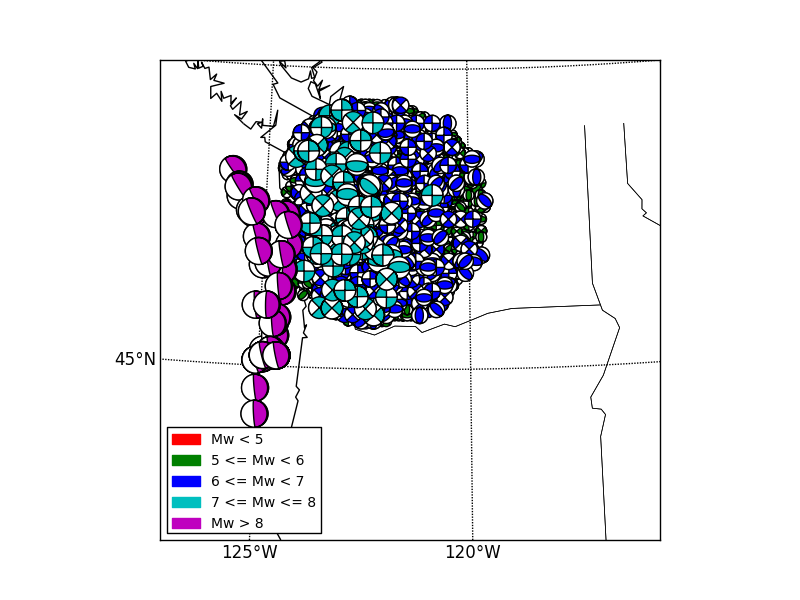
\includegraphics[width=14cm]{./Pictures/ses_USA_NSHMP2008.png}
\caption{Stochastic event set for a region surrounding Seattle (U.S.) for a duration of 10000 years.}
\label{fig:seattle_ses}
\end{figure}
\begin{figure}
\centering
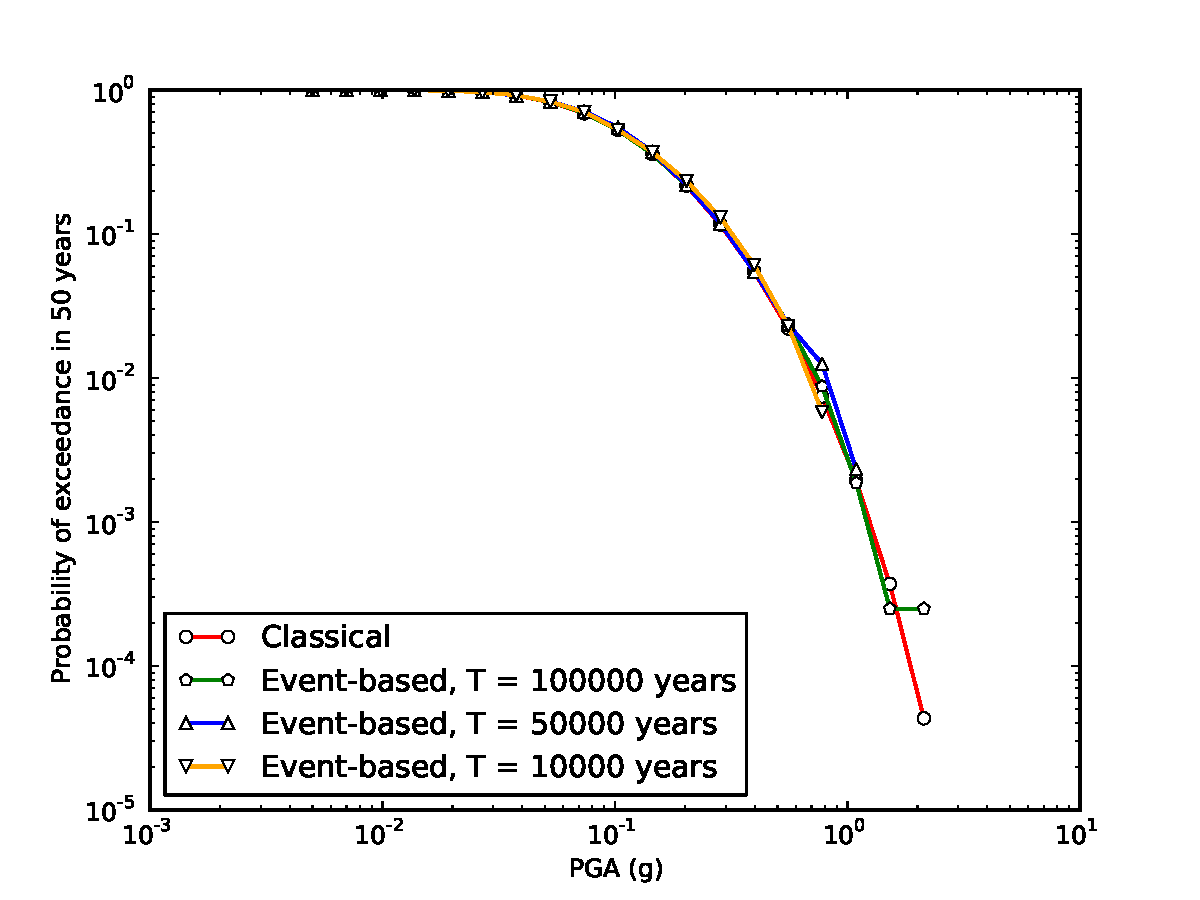
\includegraphics[width=14cm]{./Pictures/Seattle.pdf}
\caption{Hazard curves for Seattle using the Classical and Event-based approaches.}
\label{fig:seattle_curves}
\end{figure}

\section{Disaggregation analysis}
We present here an example of disaggregation analysis for the city of Seattle, always considering the 2008
national seismic hazard model for U.S. developed by (CITE PERTERSEN). In particular, we show the geographic-magnitude (Figure \ref{fig:seattle_lonlatmag}) and geographic-tectonic region type (Figure \ref{fig:seattle_lonlattrt}) disaggregation histograms for PGA corresponding to 10\% probability of exceedance in 50 years. The geographic disaggregation allows investigating the spatial distribution of the
seismic sources contributing to a given level of hazard. By including magnitude and tectonic region type,
we can understand the influence of the different tectonic regions, and also the magnitude ranges involved.
Indeed, the disaggregation analysis for the city of Seattle shows that, for a return period of 475 years, the
highest probabilities of ground motion exceedance are associated with active shallow crust events with magnitudes in the range 6 to 7. The second highest contributions are from subduction interface events
with magnitudes above 9. Subduction intraslab events are instead associated to the lowest contributions.
\begin{figure}
\centering
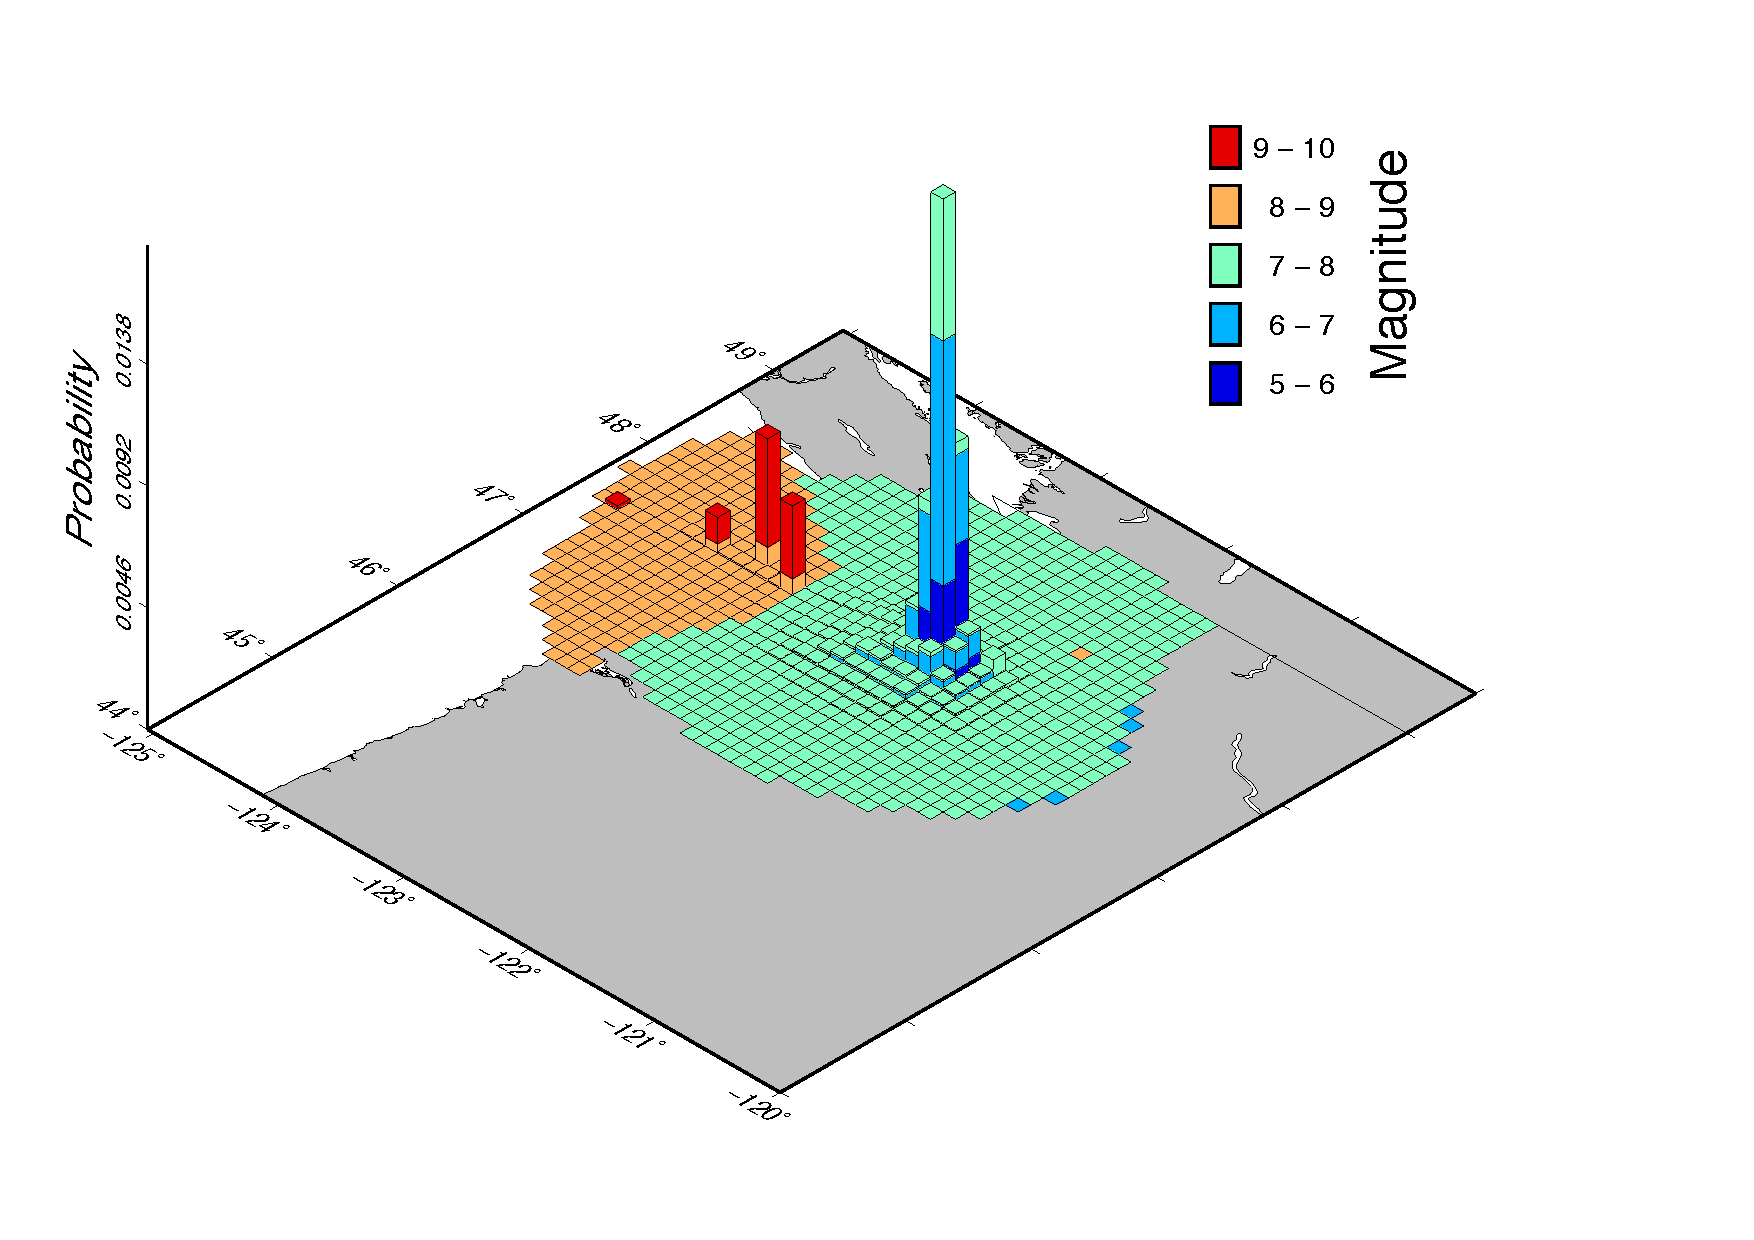
\includegraphics[width=14cm]{./Pictures/Seattle_Lon_Lat_Mag.pdf}
\caption{Longitude, latitude and magnitude disaggregation for PGA corresponding to 10\% probability of exceedance in 50 years.}
\label{fig:seattle_lonlatmag}
\end{figure}

\begin{figure}
\centering
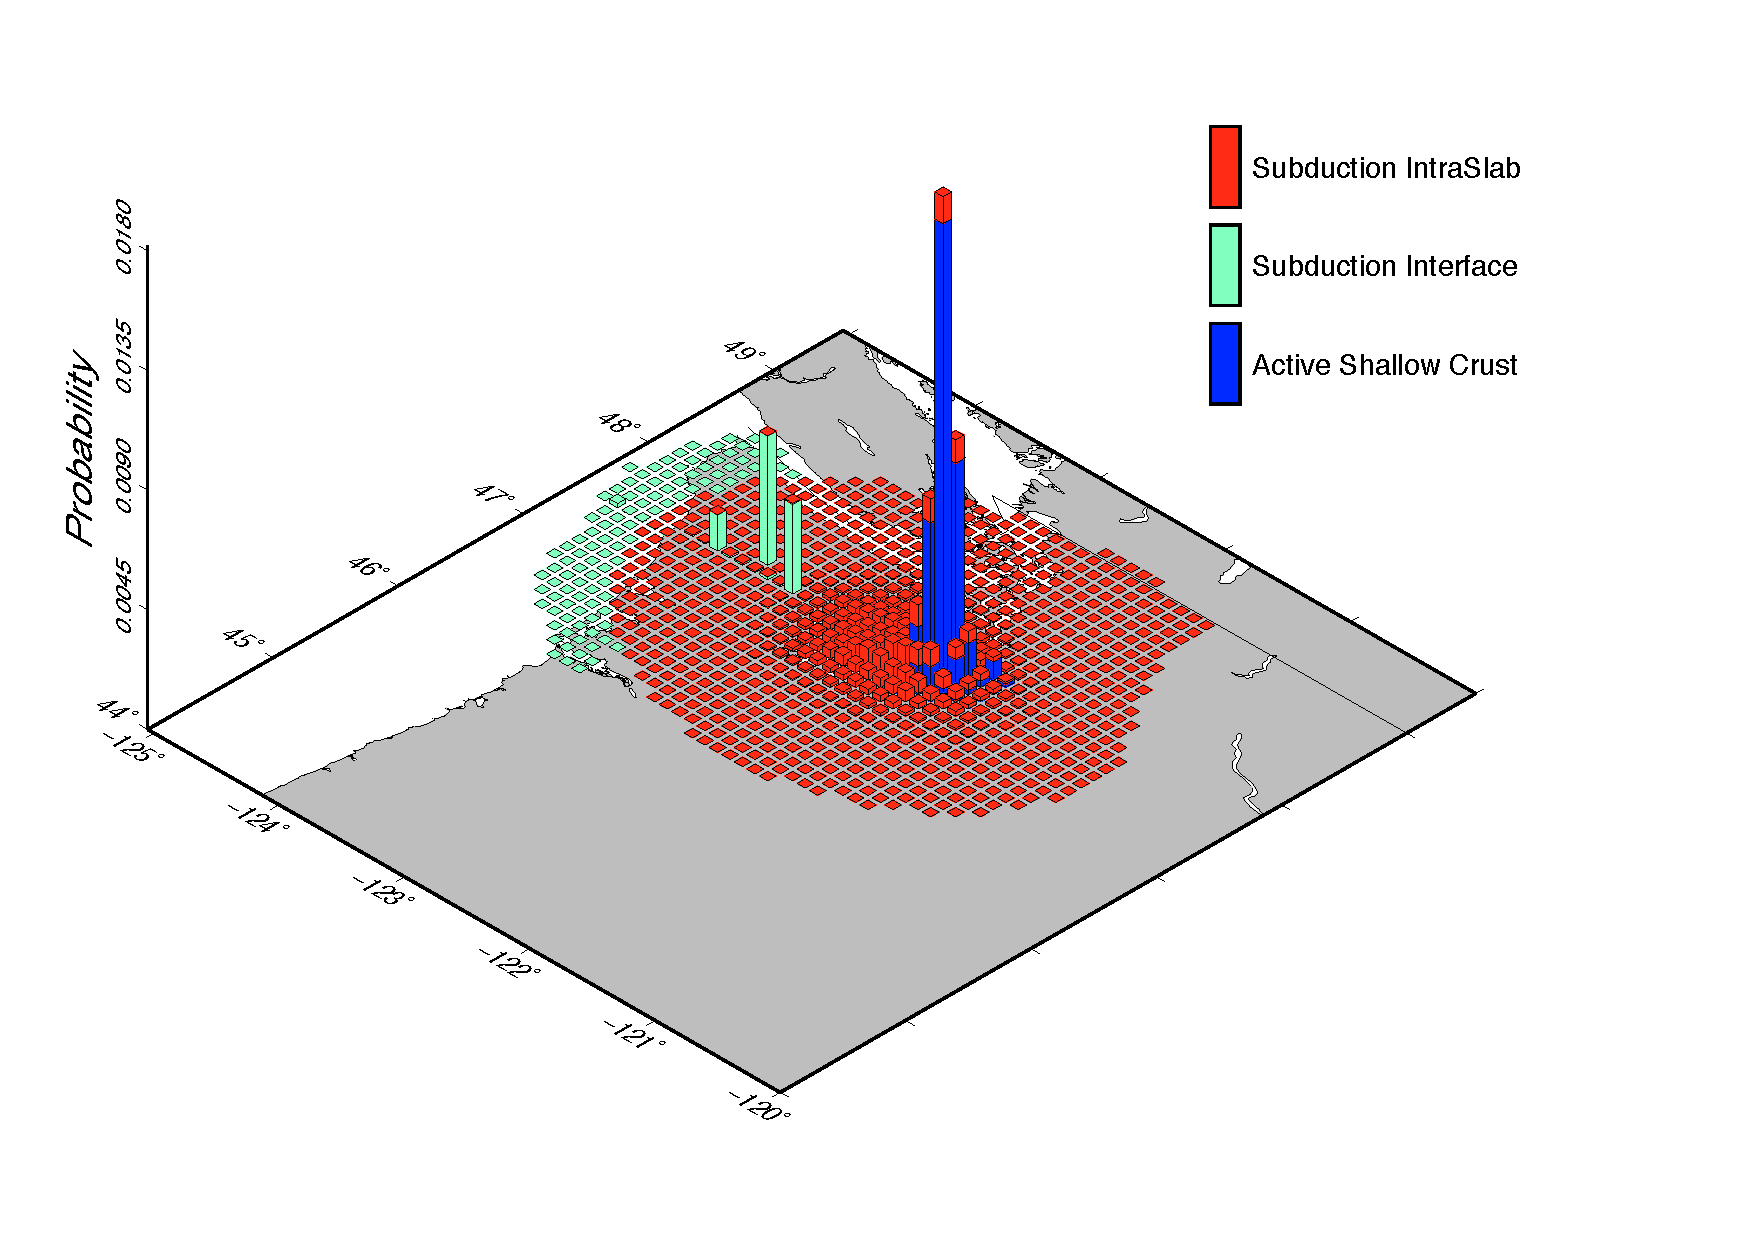
\includegraphics[width=14cm]{./Pictures/Seattle_Lon_Lat_TRT.pdf}
\caption{Longitude, latitude and tectonic region type disaggregation for PGA corresponding to 10\% probability of exceedance in 50 years.}
\label{fig:seattle_lonlattrt}
\end{figure}

